\section{Task 4: Insecure Network Services} \label{ch:pentesting:network-services}
This section covers the network services found in the system and their implications on the system's security. As rated by OWASP, this is the second most common source of security issues within IoT systems \cite{owasp-iot-top10}, see section \ref{ch:related-work:owasp}.

\subsubsection{Background}
During development, many manufacturers deploy network services on IoT devices for remote debugging. However, a very common source of vulnerabilities is leaving these network services active on live devices shipped to customers \cite{owasp-iot-top10}. This could be done in negligence or on purpose to leave a backdoor for the manufacturer to debug live devices. These services could for example be a telnet or SSH server. This combined with weak passwords is an all too common occurrence in IoT systems \cite{understanding-mirai}. This is such a common issue that OWASP ranks it the second most common source of security issues in IoT devices \cite{owasp-iot-top10}. Additionally, the ETSI EN 303 645 standard explicitly mentions minimizing the system's attack surface, in provision 6, by removing unnecessary network services \cite{etsi-iot-standard} (see section \ref{ch:related-work:etsi}).

Often such services are completely unnecessary for the functionality of the system and only serve to increase its attack surface. Even when they are protected by a strong password it can sometimes be found by analyzing the firmware. Additionally, the system can be vulnerable due to vulnerabilities present in the network service itself, the protocol used, or the OS network stack. Additionally, these systems are often using outdated versions of said services, potentially leaving the system exposed to publicly disclosed vulnerabilities. This is so common that OWASP ranks it as the fifth most common source of vulnerabilities for IoT systems \cite{owasp-iot-top10}.

\subsubsection{Method}
Initially, which network services the system hosts had to be identified. This was done using the open-source network scanning tool \textit{Nmap}\footnotelink{https://nmap.org/}{2021-05-25}. First, the basic port scanning functionality of Nmap was launched against the system, using the following command:
\begin{lstlisting}[frame=tb]
    nmap -p- $IP
\end{lstlisting}
This scans the device for processes listening on all TCP ports in the entire 0-65535 range. Similarly, a scan was made on UDP ports as well. However, due to the known difficultly of UDP port scans, only the most common UDP ports were scanned, as a scan of the full port range was estimated to take several weeks. This was done using the following command:
\begin{lstlisting}[frame=tb]
    sudo nmap -sU -F -v $IP
\end{lstlisting}
The UDP scan showed no active services except a DNS server on port 53. However, the TCP showed three network services listening on different ports on the device. The following network services were identified:
\begin{itemize}
    \item 53/udp: A DNS server.
    \item 53/tcp: A DNS server.
    \item 80/tcp: The local admin server, as described in section \ref{ch:system:local-admin}.
    \item 58098/tcp: An unknown process listening in an unconventional port.
\end{itemize}
The web server listening on port 80 provides very little functionality, as described in section \ref{ch:system:local-admin}. It features a login form. An unsuccessful password attack was conducted against this form, see section \ref{ch:pentesting:password}. From the \textit{Server} HTTP header, however, it leaks information about which web server is used.

To gain more information about these services a version detection scan was launched against the three ports, using the following command:
\begin{lstlisting}[frame=tb]
    nmap -sV --version-all -p53,80,58098 $IP
\end{lstlisting}
The Nmap version detection scan took around 10 minutes and yielded no result for the unknown application running on port 58098 or any further information about the other two services. To further investigate information about the process the open-source application scanner \textit{Amap}\footnotelink{https://github.com/BlackArch/amap}{2021-05-26} was used. This is a lesser-known program created by the prolific hacker group \textit{The Hacker's Choice}\footnotelink{https://www.thc.org/}{2021-05-26}. According to the authors, the Amap application scanner has largely been superseded by Nmap. Thus unsurprisingly, it provided no additional information about the services. However, the application suite includes a very simple TCP fuzzer called \textit{Amapcrap}. This is a program that sends random bytes to an open TCP port to elicit a response from an otherwise silent application, which can be very useful in black box testing an opaque network service. This was tried against the system using the following command:
\begin{lstlisting}[frame=tb]
    amapcrap $IP 58098
\end{lstlisting}

\subsubsection{Results}
The result of the full port scan shows three active services on the device:
\begin{itemize}
    \item A DNS server, running on the standard DNS ports, \textit{53/tcp} and \textit{53/udp}.
    \item A web server, \textit{80/tcp}, the functionality of which is covered in section \ref{ch:system:local-admin}.
    \item An unknown application, running on \textit{58098/tcp}.
\end{itemize}
Additionally, the application and version scanners that were run against the services gave no information at all about the three services. The \texttt{Server} HTTP header returned from the webserver, however, leaked the fact that it uses an open-source web server for embedded systems called \textit{Mongoose}\footnotelink{https://github.com/cesanta/mongoose}{2021-06-07}.

Lastly, fuzzing the unknown service, \textit{58098/tcp}, using the \textit{AmapCrap} tool, made the service unresponsive. This is shown in figure \ref{fig:amapcrap-fuzz-attack}. Presumably, the application crashed on this specific input.
\begin{figure}[!ht]
    \centering
    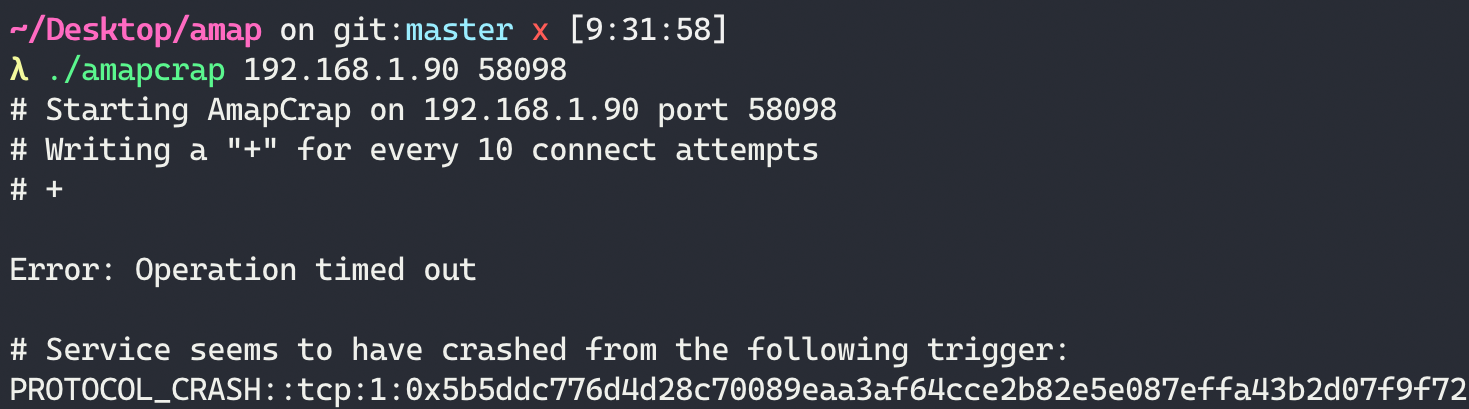
\includegraphics[width=\textwidth]{images/6-pentesting/amapcrap-fuzz-crash.png}
    \caption{The 58098/tcp application crashing during a fuzzing attack.}
    \label{fig:amapcrap-fuzz-attack}
\end{figure}

Examining the input further reveals that the first two bytes represent the characters \texttt{[]} in ASCII, which is intriguing. Through manual testing using telnet on the correct port and trial and error, it was discovered that the application crashed on more inputs. These include \texttt{\{\}} and \texttt{[1,2,3]}, for example. While the application presumably crashes and becomes temporarily unresponsive, the system seems to automatically revive the process. Within about a minute it starts accepting TCP connections again. None of the other functionality of the system is seemingly affected during this downtime, however.

\subsubsection{Discussion}
Performing a network scan on the system revealed three network services listening on three different TCP ports. However, no vulnerabilities were found as a result of these three services. The purpose of the first one, the DNS server, is quite unclear. There is seemingly no self-hosted domain documented anywhere so why the system hosts a DNS server is as of now unknown. The second server, the HTTP web server, has been covered at length in section \ref{ch:system:local-admin}, as well as a pentest that was launched against it which is covered in section \ref{ch:pentesting:password}. The third server is the most interesting find from this section. It is hosted on an unconventional TCP port, presumably to hide it slightly from attackers. The application is completely opaque and does not seem to react at all to most inputs. Through all fuzzing and manual testing, the application never sent a single response over the TCP connection. However, though fuzzing several inputs were found that seemingly crash the server. The pattern of said inputs suggests that the server might be trying to parse JSON and crashing when the input is of an unexpected format. It could perhaps be a successful \gls{DOS} attack against the system. However, the purpose of this service is unclear and seemingly no functionality of the system is negatively affected while this application is unresponsive.

A guess as to the functionality of this server is an obfuscated backdoor to the system. Instead of a standard telnet server, it might be hidden behind an application that expects a specific string. Only when it receives it does the remote shell launch. However, as it stands currently the application is a complete black box. Without access to the firmware additional investigation is very difficult. It was therefore considered unfeasible and it was not investigated further.

As stated, no additional vulnerabilities were discovered as a result of this investigation into the systems network services. The more important question, however, is \textit{why}? When OWASP ranks it as the second most common source of security issues for this type of system \cite{owasp-iot-top10}, why are these network services active on the device in the first place? It is in clear violation of provision 6 of the ETSI EN 303 645 standard, urging manufacturers to minimize the attack surface. There is seemingly no reason for them to exist. If one were to discover the password to the admin web panel, for example, every aspect of the security of the system is compromised. It opens up the system to potentially critical vulnerabilities. Climax Technology have already made this mistake at least once before. Researchers investigating a similar system from the same manufacturer discovered a telnet server listening on a similar unconventional high port. By analyzing the firmware they found that the root password could be derived simply from the panels MAC address \cite{labvienna} (see section \ref{ch:related-work:lupus}), giving them complete control over the system. This is a typical example of both the number one spot in the OWASP IoT top 10, and a violation of the first provision of the ETSI EN 303 645 standard.

Unfortunately, the firmware of the system in this thesis was not found publicly available. It was decided to be outside the scope of this thesis but if one were to, for example, solder off the flash memory from the main panel's PCB and read its contents one could get access to the firmware. It is not unlikely that through reverse-engineering the firmware one could find the password to the local admin panel or understand more about how the \textit{58098/tcp} application works and what its purpose is. This could lead to additional \textit{critical} vulnerabilities. The fact is that these services are seemingly not needed for the functionality of the system, and only serve to increase the attack surface of the system, is worrying and in clear contradiction of the ETSI EN 303 645 standard \cite{etsi-iot-standard}.
